\section{Assignment}

\subsection{Q-1: Boston Housing}

\subsubsection*{(a) Explore the Boston dataset in MASS library}
The Boston data frame has 506 rows and 14 columns. The data set contains different properties about suburbs of Boston. The types of data are integers and numerics. 


\begin{figure}[H]
\centering
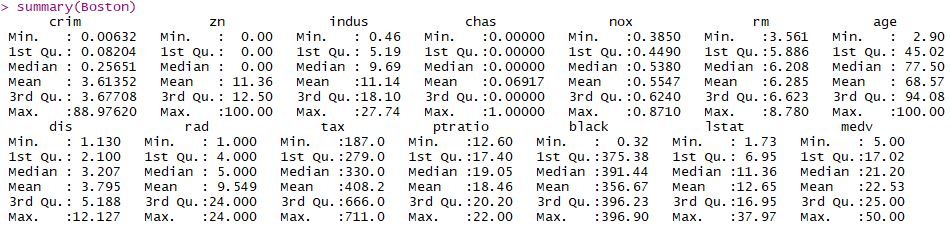
\includegraphics[scale=0.49]{Graphics/Assignment1/ExploreBoston.JPG}
\caption{Descriptive overview of Boston dataset}
\label{fig:logistic_regression_confusions_matrix_001}
\end{figure}


\subsubsection*{(b) Fit classification models}
\textbf{Logistic regression}





\iffalse
Step 1: Load data and run numerical and graphical summaries\\
Step 2: Split the data into training and testing data \\
Step 3: Fit a logistic regression model using training data\\
Step 4: Use the fitted model to do prediction for the test data\\
Step 5: Create the confusion matrix and compute the misclassification rate\\ \\
\fi


In figure \ref{fig:generalized_linear_model} the generalized linear model is explored. The features which are the most significant should be explored further. The algorithm outputs significant codes which results in the features with lowest p-values. The p-value expresses whether the null hypothesis should be accepted or rejected. If the the p-value is less or equal to the significance level, there is strong evidence to reject the null hypothesis and accept the alternative hypothesis, $H_A$.   
In this case, the hypothesis expresses the influence of the predictor features to the predicted feature, which is the 'crim01'. The null hypothesis will be expressed as follows: $H_0 = 0$. 

The $H_0 = 0$  states that a specific predictor feature doesn't have a strong association to the predicted feature. To find the features with importance to the predicted value, the null hypothesis has to be rejected, hence using the p-value.    


\begin{figure}[H]
\centering
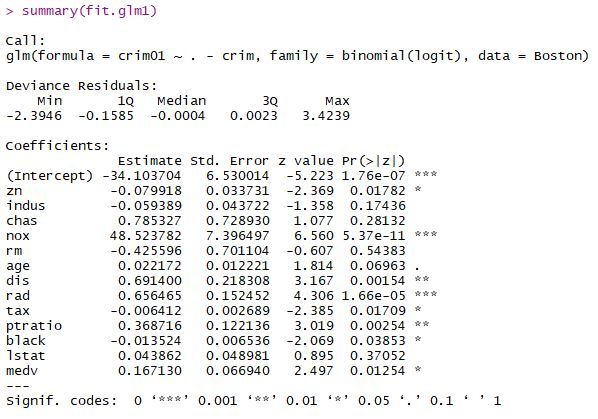
\includegraphics[scale=0.65]{LogisticRegressionCoefficientsExplore.JPG}
\caption{Generalized linear model}
\label{fig:generalized_linear_model}
\end{figure}

From the exploratory model, the following features which have a strong influence to the predicted value are: zn, nox, dis, rad, tax, ptratio, black and medv. 
All of these features are at a significance level of 0.05. In this experiment, other subsets of features will be used with different significance level. There are three subsets with different significance levels, 0.05, 0.01 and 0.001. The following features are at a significance level equal or less than 0.01: nox, dis, rad and ptratio. The last subset is for a significance level of 0.001: nox and rad.  

The misclassification of the models are computed with respect to the different subsets and their features with the training data as data input. Each model results in a confusion matrix. From the confusion matrix the misclassification rate and accuracy is computed by using formula from figure \ref{fig:confusion_Matrix} in the appendix. The predict function computes the predicted probabilities for crime based on the test data. The predicted probabilities are used to compute if the crime rate is above or below the median. The figures \ref{fig:logistic_regression_confusions_matrix_005}, \ref{fig:logistic_regression_confusions_matrix_001} and \ref{fig:logistic_regression_confusions_matrix_0001} shows the different confusion matrices and error rates for each training of model in respect to their significance level.  \\

\begin{figure}[h]
\centering
\begin{minipage}{0.32\textwidth}
\centering
    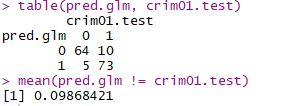
\includegraphics[width=\linewidth, height= 60pt]{LogisticRegressionConfusionsMatrix.JPG}
    \caption{Confusion Matrix - sign. level of 0.05}
    \label{fig:logistic_regression_confusions_matrix_005}
\end{minipage}\hfill
\begin{minipage}{0.32\textwidth}
\centering

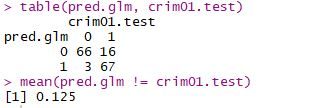
\includegraphics[width=\linewidth, height= 60pt]{LogisticRegressionConfusionsMatrix_001.JPG}
    \caption{Confusion Matrix - sign. level of 0.01}
    \label{fig:logistic_regression_confusions_matrix_001}
\end{minipage}\hfill
\begin{minipage}{0.32\textwidth}
\centering

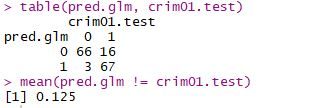
\includegraphics[width=\linewidth, height= 60pt]{LogisticRegressionConfusionsMatrix_001.JPG}
    \caption{Confusion Matrix - sign. level of 0.001}
    \label{fig:logistic_regression_confusions_matrix_0001}
\end{minipage}
\end{figure}


\noindent
\textbf{Linear Discriminant Analysis} \\
In the following experiment with Linear Discriminant Analysis (LDA), the same features with respect to the significance levels will be used for the model training. Just as before, each model has a confusion matrix and error rate. From the results, each feature has a coefficient, which determine the process growth.

Some of the coefficients are negative and some are positive. Negative coefficients indicate the larger the feature the less is the crime rate. The value of said feature determines the influence or the effect on the crime rate. So, the larger the coefficient the more it affects the crime rate. 

\begin{figure}[H]
\centering
\begin{minipage}{0.32\textwidth}
\centering
    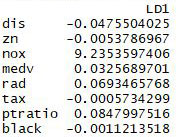
\includegraphics[width=\linewidth]{Graphics/Assignment1/LDACoefficients_005_1.jpg}
    \caption{LDA Coefficients - sign. level 5\%}
    \label{fig:LDA_005}
\end{minipage}\hfill
\begin{minipage}{0.32\textwidth}
\centering

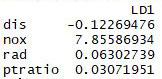
\includegraphics[width=\linewidth, height= 50pt]{Graphics/Assignment1/LDACoefficients_001_1.jpg}
    \caption{LDA Coefficients - sign. level 1\%}
    \label{fig:LDA_001}
\end{minipage}\hfill
\begin{minipage}{0.32\textwidth}
\centering

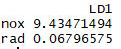
\includegraphics[width=\linewidth, height=25pt]{Graphics/Assignment1/LDACoefficients_0001_1.jpg}
    \caption{LDA Coefficients - sign. level 0.1\%}
    \label{fig:LDA_0001}
\end{minipage}
\end{figure}

The figures \ref{fig:LDA_005}, \ref{fig:LDA_001} and \ref{fig:LDA_0001} shows the different confusion matrices and error rates for each training of model in respect to their significance level. 

\begin{figure}[H]
\centering
\begin{minipage}{0.32\textwidth}
\centering
    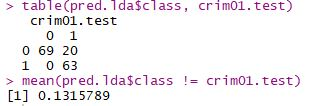
\includegraphics[width=\linewidth, height=50pt]{Graphics/Assignment1/LDAConfusionsMatrix_005.JPG}
    \caption{LDA Confusion Matrix - sign. level 5\%}
    \label{fig:LDA_005}
\end{minipage}\hfill
\begin{minipage}{0.32\textwidth}
\centering

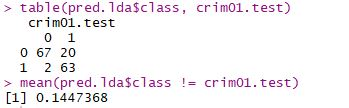
\includegraphics[width=\linewidth, height= 50pt]{Graphics/Assignment1/LDAConfusionsMatrix_001.JPG}
    \caption{LDA Confusion Matrix - sign. level 1\%}
    \label{fig:LDA_001}
\end{minipage}\hfill
\begin{minipage}{0.32\textwidth}
\centering

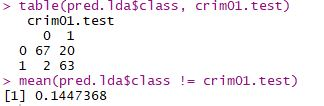
\includegraphics[width=\linewidth, height= 50pt]{Graphics/Assignment1/LDAConfusionsMatrix_0001.JPG}
    \caption{LDA Confusion Matrix - sign. level 0.1\%}
    \label{fig:LDA_0001}
\end{minipage}
\end{figure}


\noindent
\textbf{K-Nearest Neighbors}\\
For this algorithm, the same subsets of features are used in relation to their significance level. Before the algorithm can be used with the subsets, the data has to be normalized and the optimal \textit{k} values need to be found. In the process of finding the optimal \textit{k's}, a list of \textit{k's} have been evaluated by using the \textit{class} package in R. It enables the use of the method \textit{knn()}. The optimal \textit{k's} will be decided on their accuracy rates. Figure \ref{fig:optimal_ks} shows a plot between best accuracy and the optimal number of \textit{k's}. The optimal \textit{k's} in the experiment are 3 and 5. 

\begin{figure}[H]
\centering
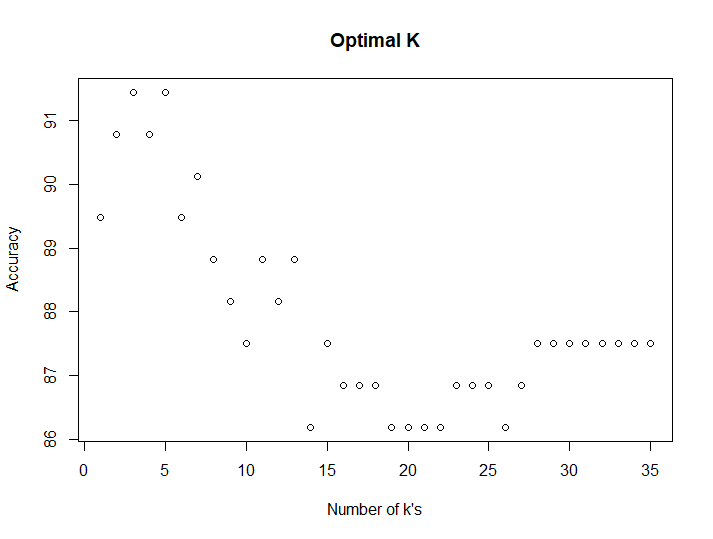
\includegraphics[scale=0.65]{Graphics/Assignment1/Rplot.png}
\caption{Plot of all k's}
\label{fig:optimal_ks}
\end{figure}


\subsubsection*{(c) Description of the findings}

\begin{itemize}
    \item What are the models test error rates?
    \item Which model offers the best prediction?
    \item What are the relevant observed variables to consider?
\end{itemize}



\begin{table}[H]
\centering
\begin{tabular}{|c|c|c|c|}
\hline
Algorithm           & \begin{tabular}[c]{@{}c@{}}Significance \\ Level (\%)\end{tabular} & Accuracy (\%)                                                   & \begin{tabular}[c]{@{}c@{}}Misclassification \\ error rate (\%)\end{tabular} \\ \hline
Logistic Regression & 5                                                                  & 90.14                                                           & 9.86                                                                         \\ \hline
Logistic Regression & 1                                                                  & 87.5                                                            & 12.5                                                                         \\ \hline
Logistic Regression & 0.1                                                                & 88.2                                                            & 11.8                                                                         \\ \hline
LDA                 & 5                                                                  & 86.9                                                            & 13.1                                                                         \\ \hline
LDA                 & 1                                                                  & 85.2                                                            & 14.4                                                                         \\ \hline
LDA                 & 0.1                                                                & 85.5                                                            & 14.4                                                                         \\ \hline
KNN                 & 5                                                                  & \begin{tabular}[c]{@{}c@{}}(k=3) 93.2\\ (k=5) 92.8\end{tabular} & \begin{tabular}[c]{@{}c@{}}(k=3) 6.8\\ (k=5) 7.2\end{tabular}                \\ \hline
KNN                 & 1                                                                  & \begin{tabular}[c]{@{}c@{}}(k=3) 96.1\\ (k=5) 95.4\end{tabular} & \begin{tabular}[c]{@{}c@{}}(k=3) 3.9\\ (k=5) 4.6\end{tabular}                \\ \hline
KNN                 & 0.1                                                                & \begin{tabular}[c]{@{}c@{}}(k=3) 94.8\\ (k=5) 93.4\end{tabular} & \begin{tabular}[c]{@{}c@{}}(k=3) 5.2\\ (k=5) 6.6\end{tabular}                \\ \hline
\end{tabular}
\caption{Accuracy and Error rate in relation to significance level}
\label{table1}
\end{table}

\iffalse
It is important to note that LDA with CV = TRUE or FALSE, results the same.
\fi

\subsection{Q-2: Students Performance}

\subsubsection*{(a) Explicit model and probability for scoring an A}

To create an explicit model $L(\textbf{x})$ is calculated using the given $\beta_0$ and $\beta^T$ parameters. The \textbf{x} vector is a variable denoting the time invested in student's study and the student's grade point average. 

\begin{equation*}
    L(\textbf{x}) = \beta_0+\beta^T \textbf{x}=-6+[0.05,1]\begin{bmatrix}x_1 \\ x_2\end{bmatrix}
\end{equation*} 

The result of $L(\textbf{x})$ is put into the logistic regression model to be able to calculate probabilities of a student scoring an A at the exam. $\Pi_1$ will then represent the class of a student scoring an A and \textbf{x} a given student.

\textbf{Logistic Model:}
\begin{equation*}
\mathbb{P}(\Pi_1 | \textbf{x}) = \frac{e^{L(\textbf{x})}}{1+e^{L(\textbf{x})}} = \frac{e^{-6+[0.05,1][x_1, x_2]^T}}{1+e^{-6+[0.05,1][x_1,x_2]^T}}    
\end{equation*}

Given a student who studies 40 hours a week and has a grade point average of 3.5 (C+) the model is used to determine the probability of that student scoring an A at the exam by inserting the given information as $x_1$ and $x_2$.

\begin{equation}
\mathbb{P}(\Pi_1 | \textbf{x}) =  \frac{e^{-6+[0.05,1][40,3.5]^T}}{1+e^{-6+[0.05,1][40,3.5]^T}} =
\frac{e^{-0.5}}{1+e^{-0.5}} = 0.3775     
\end{equation}

The student has a 37.8 \% probability of getting an A at the exam.

\subsubsection*{(b) Weeks to study for 80\% chance of scoring an A}

Now the same student from the previous exercise wants to know how many hours of studying each week it will take to get a 80\% chance of getting an A to the exam.
To calculate the number of studying hours a week the probability of the logistic model is set to 0.8 and $L(\textbf{x})$ is isolated. Afterwards $x_1$, denoting weakly studying hours, will be isolated in the equation of $L(\textbf{x})$. 

\begin{align*}
\mathbb{P}(\Pi_1 | \textbf{x}) = \frac{e^{L(\textbf{x})}}{1+e^{L(\textbf{x})}} &= 0.8 \\
e^{L(\textbf{x})} &= 0.8*(1+e^{L(\textbf{x})}) \\
e^{L(\textbf{x})} &= 0.8 + 0.8*e^{L(\textbf{x})} \\
-0.8 &= 0.8*e^{L(\textbf{x})} - e^{L(\textbf{x})} \\ 
-0.8 &= -0.2*e^{L(\textbf{x})} \\
\frac{-0.8}{-0.2} &= e^{L(\textbf{x})} \\
ln(\frac{-0.8}{-0.2}) &= L(\textbf{x}) = 1.386 \\
& \\
L(\textbf{x}) = -6+[0.05,1]\begin{bmatrix}x_1 \\ 3.5\end{bmatrix}&=1.386 \\
-6+0.05*x_1+1*3.5&=1.386\\
0.05*x_1&=1.386+6-3.5\\
x_1=\frac{3.886}{0.05}&=77.72 hours \\
\end{align*}

A student with a grade point average of 3.5 (C+) needs to study 77.72 hours a week to have 80\% chance of scoring an A at the exam.


\section{Alcohol Related Car Crash}

\subsection{Identify demographic characteristics}
Identify the demographic characteristics of the drivers that are risk (or protective) factors of car accidents.

This is done by creating a binomial logistic model of each of the parameters, Gender, Age, Socioeconomic status, and the Accident parameter.
The results were the following:

\begin{itemize}
    \item Accident and Age: Coefficient 1.044 and confidence interval [1.026, 1.064] with p-value $3.14*10^{-6}$
    \item Accident and Gender (Male): Coefficient 4.761 and confidence interval [2.348, 10.377] with p-value $3.36*10^{-5}$
    \item Accident and Socioeconomic status: 
    \begin{itemize}
        \item Status Middle: Coefficient 1.074 and confidence interval [0.470, 2.416] with p-value $0.864$
        \item Status Upper: Coefficient 1.215 and confidence interval [0.596, 2.502] with p-value $0.592$
    \end{itemize}
\end{itemize}

From these demographics it can be seen that there is a significant association between Age and Accident, and between Gender and Accident given the significance value 0.05.

\subsection{Model}

Obtain the model relating BAC and car accidents (both, not adjusted and adjusted for confounders). 

Adjusted:
To obtain the model relating BAC and car accidents we have to check if the three conditions for the variables being a confounder. The three conditions are the following:
\begin{enumerate}
    \item Associated with BAC
    \item Risk factor for Accident (independent of BAC)
    \item Not intermediate factor (BAC is not depended on potential confounder)
\end{enumerate}
The potential confounder: Gender, Age, Socioeconomin status

In relation to condition 1, it is still not known if both "age" and "gender" are associated with BAC. To find out the association between the two potential confounders and BAC there has been done a logistic model. The results are the following:

\begin{itemize}
\item Age: Coefficient:0.011 and p-value: $2.39*10{^}-08$

\item Gender: Coefficient:0.276 and p-value: $0,167*10{^}-3$

\end{itemize}

It is now shown that condition 1 is also confirmed since the p-value is under 0.05. 

As for condition 2, it is already found out that "gender" and "age" is significant which means they are a risk factor for accident. Also it is seen that "age" and "gender" is not intermediate factors which is condition 3. We can now confirm that "age" and "gender" are confounders. 


\textbf{Model for adjusted: } 
The adjusted model is when the confounders "age" and "gender" are included: 

\begin{itemize}

\item The logarithmic coefficient of BAC is 3.78, Gender is 0.92 and Age is 0.022 with the p-value < 0.05

\item The logarithmic confidence interval of BAC is [2.77, 4.97], Gender is [-0.054, 1.93] and Age is [-0.0018, 0.047]

\item The natural coefficient of BAC is 43.76, Gender is 2.51 and Age is 1.02 and confidence interval for BAC is [15.90, 144.08], Gender is [0.95, 6.91] and Age is [1.00, 1.05]

\end{itemize}


\textbf{Model for not Adjusted:}
The not adjusted model is when only looking at BAC and accident. 

\begin{itemize}

\item The logarithmic coefficient of BAC is 4.00 with the p-value < 0.05
\item The logarithmic confidence interval is [3.03, 5.14]
\item The natural coefficient (54.70) and confidence interval [20.77, 171.21]

\end{itemize}


\textbf{Interpret the not‐adjusted and adjusted odds ratios:}

It is seen that the unadjusted model shows the BAC odds ratio is 54.7. This means that when BAC is increased by 1 the subject has 54.7 times higher odds of getting into an accident. 

The adjusted model shows that BAC odds ratio is 43.7. This means BAC is increased by 1 the subject has 43.7 times higher odds of getting into an accident. 

This shows that when taking age and gender into consideration, there is less chance to get into an accident compared to the unadjusted model. The difference is not that big, so the association does not make a extraordinary difference but it does make a different to some extend.

Is there a significant association between BAC and car accidents? 

\subsection{Other potential confounder}
Is there any other potential confounder (not included in the file ”Data\_car\_accidents”) that should have
been considered in the study? 
How would you include it in the analysis?

Some other potential confounders based on demographics could be the following:
\begin{itemize}
    \item Weight (in kilos)
    \item Vision (Good or Poor): Poor vision will be characterized as not wearing classes while driving when needing them
    \item Medication (Yes or No): Medication in this sense is characterized as medication not appropriate for driving
    
\end{itemize}
How would you include it in the analysis?

A potential confounder could be weight since BAC affects the body more the less someone weight. This factor might be an important factor in this case and also it is associated with BAC (condition 1). The "weight" factor is a risk factor for accident independent of BAC which is condition 2 and at last BAC is not depended on weight (condition 3). This explains why weight could be a confounder for this case.

Vision could also be a factor to look into. The vision might be associated with BAC(condition 1); when drinking alcohol ones vision might get affected and if the drivers vision is already poor that might give a bigger impact too. It is obvious that the vision is a risk factor for accident independent of BAC(condition 2) and at last vision is not an intermediate factor(condition 3). 

Finally another potential confounder could be medication. If a driver uses medication, it might have an impact that the user is drinking. In that way medication can be associated with BAC. Medication is also a risk factor for accident to some extend. It depends on what kind of medication the driver has taken, but there are some where you are not allowed to drive if you take that spcific medication for instance. Also BAC is not dependened on medication which is condition 3. 

Some of these potential confounders might be difficult to measure for large datasets.
All 

\subsection{Unadjusted and adjusted models}

Plot the unadjusted (crude) and adjusted models. 
Comment on the similarities or differences between the
two.

The two plots is shown below:

\begin{figure}[H]
    \centering
    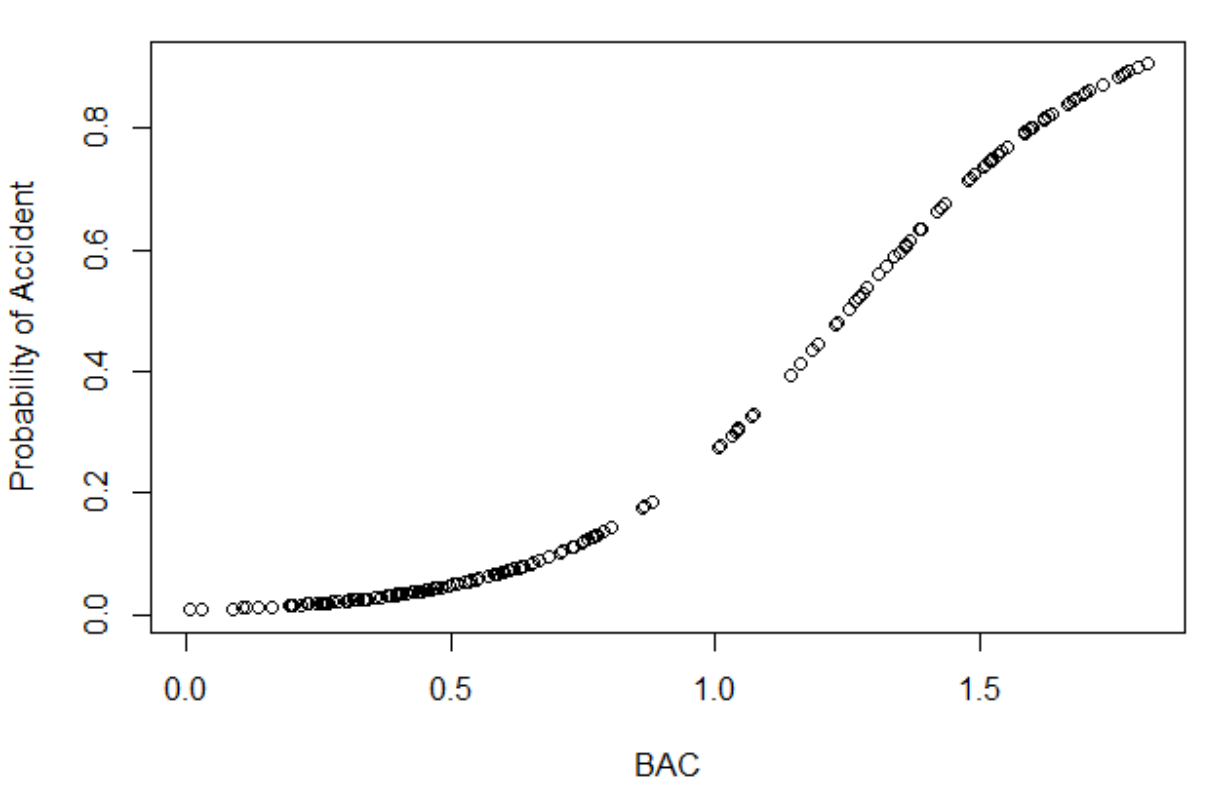
\includegraphics[scale=0.5]{unadjusted.PNG}
    \caption{Unadjusted Model}
    \label{fig:unadjusted}
\end{figure}

The unadjusted model is fitted directly to BAC as the only dependent parameter. Therefore the points fit a perfect logistic regression.

\begin{figure}[H]
    \centering
    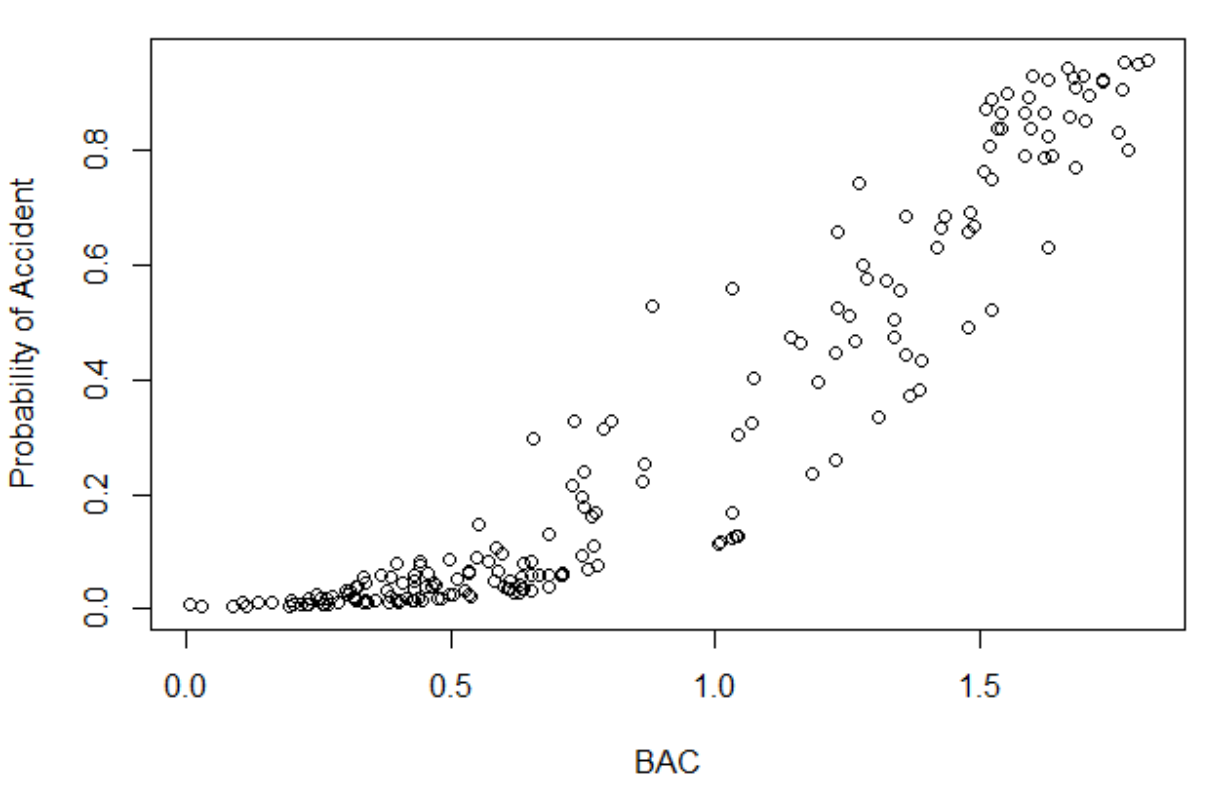
\includegraphics[scale=0.5]{adjusted.PNG}
    \caption{Adjusted Model}
    \label{fig:adjusted}
\end{figure}

The adjusted model is fitted to BAC and the two confounders, but since the plot onlyl show the dependecy of BAC, the points are not fittet as perfectly as the unadjusted model. Now the model is dependent on age and gender, which are disregarded in the plot.

In the adjusted model it can be seen that points are dense approximately below BAC on 0.6 and again it becomes slightly dense when BAC is over 1.5. This can be interpreted as when the BAC is below 0.5 and over 1.5 the model does not rely that much on the confounders, meaning age and gender does not matter when either low or high BAC.

\subsection{Probability}

What is the probability that a 40 yr male whose BAC is >1‰, causes a car accident? 

What will be the probability, 10, 20, 30 and 40 years later? Is this change linear?

Given BAC > 1.0 and Gender = Male, what is the probability of an accident (threshold = 0.5) adjusted by age.

$$
\mathbb{P}(BAC > 1) = 1 - \mathbb{P}(BAC \leq 1) = 1 - (\mathbb{P}(BAC = 0) + \mathbb{P}(BAC = 1))
$$

\begin{itemize}
    \item 40 years: P = 0.6489476 
    \item 50 years: P = 0.5940709
    \item 60 years: P = 0.5359063
    \item 70 years: P = 0.4755436 
    \item 80 years: P = 0.4141669 
\end{itemize}

\begin{figure}[H]
    \centering
    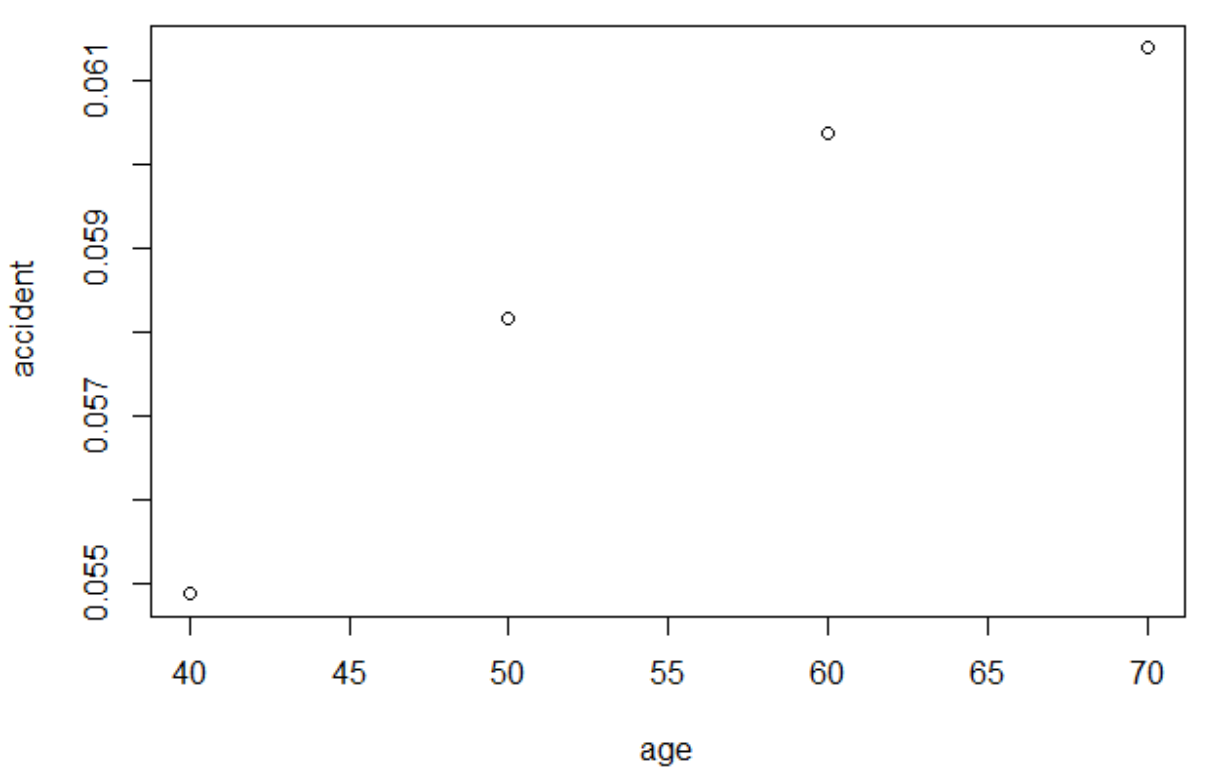
\includegraphics[scale=0.5]{difference_of_ages.PNG}
    \caption{Differences in accidents by ages}
    \label{fig:diff_ages}
\end{figure}

The change is not linear, but it looks as a logistic function.

\subsection{Predictive performance and the threshold value}

We obtain information on a new set of drivers (17 subjects). Evaluate the predictive performance of the model
by calculating the accuracy,sensitivity, specificity and precision of the model using this new data set.

Consider the threshold value for the probability as equal to 0.5. The data for the 17 subjects is in the Excel file ”

\begin{table}[H]
    \centering
    \begin{tabular}{c|c|c}
      Observed / Predicted & \textbf{Yes} & \textbf{No} \\ \hline
      \textbf{Yes} & 8 & 1 \\
      \textbf{No} & 4 & 4
    \end{tabular}
    \caption{Confusion Matrix}
    \label{tab:my_label}
\end{table}

\begin{itemize}
    \item Accuracy: (TN+TP)/(TN+FP+FN+TP) = 0.71
    \item Precision: TP/(FP+TP) = 0.8
    \item Sensitivity: TP/(TP+FN) = 0.5
    \item Specificity: TN/(TN+FP) = 0.89
\end{itemize}

\section{Artist Identification}

%------------------ Start: Chapter intro -----------------
\subsection{Results}
\label{section:Results}
Following sub chapter shows the results, firstly the image is presented and it is followed by the results and a small explanation. Snippets of source code is in the appendix, however the full source code can be found in the \textcolor{blue}{\href{https://github.com/Spiderixius/DataScienceAssignments2017/tree/master/AssignmentEsmail}{Github repository}}, which will be made public Saturday the 16th of December 2017.
% Change the link to where ever the repo will be.

%------------------ End: Chapter intro -----------------


%------------------ Start: Image 1 -----------------
\subsubsection*{Image 1}

\begin{table}[H]
    \centering
    \caption{Predictions for Figure \ref{fig:renoir}.}
    \label{tbl:renoir_predictions}
    \begin{tabular}{lllll}
    \cline{1-4}
    \multicolumn{1}{|l|}{Renoir}         & \multicolumn{1}{l|}{Manet}          & \multicolumn{1}{l|}{Degas}          & \multicolumn{1}{l|}{Monet}          &  \\ \cline{1-4}
    \multicolumn{1}{|l|}{9.16161060e-01} & \multicolumn{1}{l|}{4.37439530e-06} & \multicolumn{1}{l|}{8.38107169e-02} & \multicolumn{1}{l|}{2.37891982e-05} &  \\ \cline{1-4}
                                         &                                     &                                     &                                     &  \\
                                         &                                     &                                     &                                     & 
    \end{tabular}
\end{table}


As seen in table \ref{tbl:renoir_predictions} we can see 9.16161060e-01 which is a 91.61\% certainty that it is a Renoir painting. Therefore the painting has been classified as drawn by Renoir.
%------------------ End: Image 1 -----------------



%------------------ Start: Image 2 -----------------
\subsubsection*{Image 2}

\begin{table}[H]
    \centering
    \caption{Predictions for Figure \ref{fig:outlier}.}
    \label{tbl:outlier_predictions}
    \begin{tabular}{lllll}
    \cline{1-4}
    \multicolumn{1}{|l|}{Renoir}         & \multicolumn{1}{l|}{Manet}          & \multicolumn{1}{l|}{Degas}          & \multicolumn{1}{l|}{Monet}          &  \\ \cline{1-4}
    \multicolumn{1}{|l|}{6.23026741e-10} & \multicolumn{1}{l|}{8.16067636e-01} & \multicolumn{1}{l|}{4.14584717e-03} & \multicolumn{1}{l|}{1.79786533e-01} &  \\ \cline{1-4}
                                         &                                     &                                     &                                     &  \\
                                         &                                     &                                     &                                     & 
    \end{tabular}
\end{table}

As seen by table \ref{tbl:outlier_predictions} we can see 8.16067636e-01 which is a 81.60\% certainty that it is a Manet painting. This is however not true as the painting was painted by Jackson Pollock, but such classification is not available in the output classifier, therefore it picks the next best thing, which seems to be Manet in this case. 
%------------------ End: Image 2 -----------------


%------------------ Start: Image 3 -----------------
\subsubsection*{Image 3}

\begin{table}[H]
    \centering
    \caption{Predictions for Figure \ref{fig:manet}.}
    \label{tbl:manet_predictions}
    \begin{tabular}{lllll}
    \cline{1-4}
    \multicolumn{1}{|l|}{Renoir}         & \multicolumn{1}{l|}{Manet}          & \multicolumn{1}{l|}{Degas}          & \multicolumn{1}{l|}{Monet}          &  \\ \cline{1-4}
    \multicolumn{1}{|l|}{2.28641890e-14} & \multicolumn{1}{l|}{1.00000000e+00} & \multicolumn{1}{l|}{1.85917379e-08} & \multicolumn{1}{l|}{4.80035141e-08} &  \\ \cline{1-4}
                                         &                                     &                                     &                                     &  \\
                                         &                                     &                                     &                                     & 
    \end{tabular}
\end{table}

As seen by table \ref{tbl:manet_predictions} we can see a whooping 1.00000000e+00 which is a 100\% certainty that it is a Manet painting. Therefore the painting has been classified as drawn by Manet.
%------------------ End: Image 3 -----------------



%------------------ Start: Image 4 -----------------
\subsubsection*{Image 4}

\begin{table}[H]
    \centering
    \caption{Predictions for Figure \ref{fig:degas}.}
    \label{tbl:degas_predictions}
    \begin{tabular}{lllll}
    \cline{1-4}
    \multicolumn{1}{|l|}{Renoir}         & \multicolumn{1}{l|}{Manet}          & \multicolumn{1}{l|}{Degas}          & \multicolumn{1}{l|}{Monet}          &  \\ \cline{1-4}
    \multicolumn{1}{|l|}{4.24926483e-10} & \multicolumn{1}{l|}{4.80975071e-03} & \multicolumn{1}{l|}{9.95190263e-01} & \multicolumn{1}{l|}{1.43515150e-13} &  \\ \cline{1-4}
                                         &                                     &                                     &                                     &  \\
                                         &                                     &                                     &                                     & 
    \end{tabular}
\end{table}


As seen in table \ref{tbl:degas_predictions} we can see a 9.95190263e-01 which is a 99.51\% certainty that it is a Degas painting. Therefore the painting has been classified as drawn by Degas.


%------------------ End: Image 4 -----------------



%------------------ Start: Solution Approach --------------
\subsection{Solution Approach}
The following section briefly describes the process that was committed to get the results for section \ref{section:Results}\\

\noindent{\textbf{Gather data:}} Data was gathered using a small Bash script [\ref{code:fetch_images}] to quickly download images for a certain artist. This process was repeated for all four artists.\\

\noindent{\textbf{Explore data:}} Gathered data was explored and it was apparent that Manet did not have more than 200 images. This information lead to the decision to use a maximum of 196 images for each artist, excluding the images from the assignment and a couple of images with errors in them. The reason to that was to prevent an artist from being too dominant. An example for a dominant factor would be using 1300 images which Renoir has within the style of impressionism. The 196 images for each artist was put into their own folders, with the artist name as the folder name.\\

\noindent{\textbf{Preparing the data:}} Gathered data was then prepared, for this Python was used. The code [\ref{code:load_data}] iterates through each four folders and process the images one by one. The dimension of the images is set to 224x224 which is a good balance between detailed and size to process. Afterwards the data was shuffled within each artist (not cross shuffle among artists) afterwards split into 80\% training data and 20\% test data [\ref{code:shuffle_and_split_data}]. The training and test data is then used for training and testing the convolutional neural network model.\\

\noindent{\textbf{Picking a pre-trained network:}} To avoid having to create a convolutional neural network from scratch it was decided to make use of an existing neural network. For this VGG16 [\cite{DBLP:journals/corr/SimonyanZ14a}] has been used that was pre-trained on ImageNet[\cite{imagenet_cvpr09}]. VGG16 consists of 16 convolutional neural networks.\\

\noindent{\textbf{Transfer Learning with VGG16:}} As mentioned in the previous paragraph an existing model is used, this is to avoid having to train the convolutional neural network from scratch and since there is only a maximum of 196 images per artist. Therefore transfer learning is made use of [\ref{code:model_creation_and_training}]. This happens in the following steps:
\begin{enumerate}
    \item Adjust image input to 224x224, the same dimension as our images from preprocessing
    \item Load VGG16 model pre-trained on ImageNet [\ref{fig:imagenet_vgg16}]
    \item Take VGG16's block5\_pool layers output.
    \item Feed the block5\_pool output to freshly created flatten layer.
    \item Create two fully connected layers with 128 neurons each, using RELU activation as the synapse.
    \item Create an output layer for four classes that makes use of softmax as the classifier
    \item Freeze all the layers except the newly added layers, this is to prevent the weights changing in the remaning layers
    \item Compile the new model which can then be used for training and test. [\ref{fig:custom_vgg16}]
    \item Train the model on the 80\% training data and then evaluate the model on the 20\% test data.
\end{enumerate}

The model is now ready to be used for classification of paintings that are not part of the test and training data. The model has an accuracy of 81.63\%. Not exactly the best to classify benign vs malignant tumor, however good enough for art :)



%------------------ End: Solution Approach --------------

